\section{Dataset 1: Diabetes Dataset (Regression)}

Fuzzy C-Means Clustering was applied with a range of values for the number of clusters of 2 to 10 with an increment of 1 and the fuzziness coefficient was varied between 1.5 and 2.5 with an increment of 0.1. The results were evaluated using the Fuzzy Partition Coefficient (FPC) and culminated in a number of 2 clusters and a fuzziness coefficient of 1.5 achieving a FPC of 0.939724280208228.

The resulting TSK model achieved a MSE of 2534.134033203125.

\begin{figure}[h!]
    \centering
    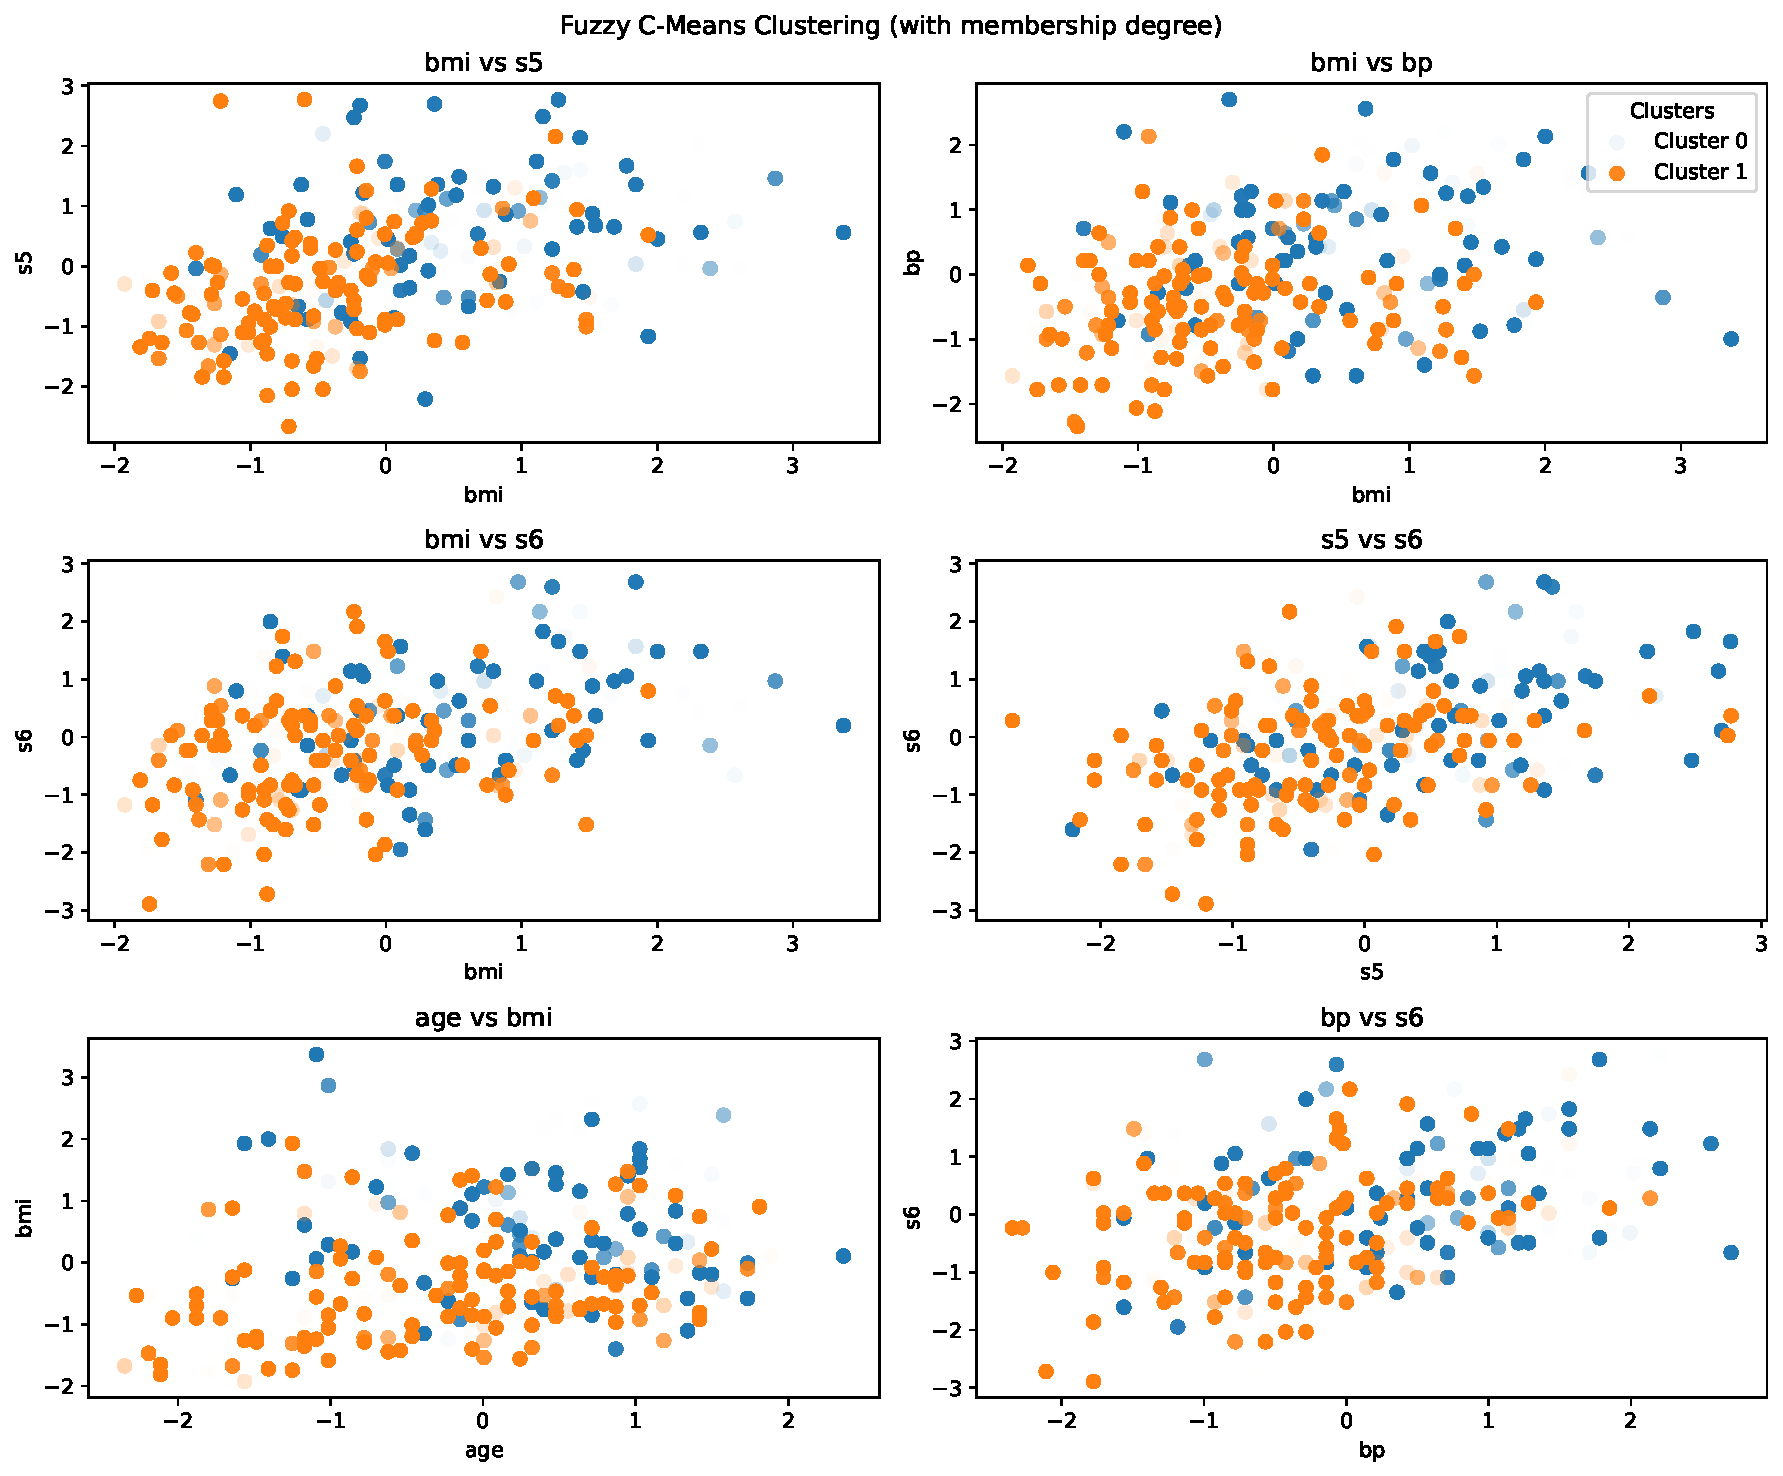
\includegraphics[width=1\textwidth]{Plots/Fuzzy C-Means Clustering (with membership degree) REG.pdf}
    \caption{Fuzzy C-Means Clustering (with membership degree)}
    \label{fig:my_label}
\end{figure}

\begin{figure}[h!]
    \centering
    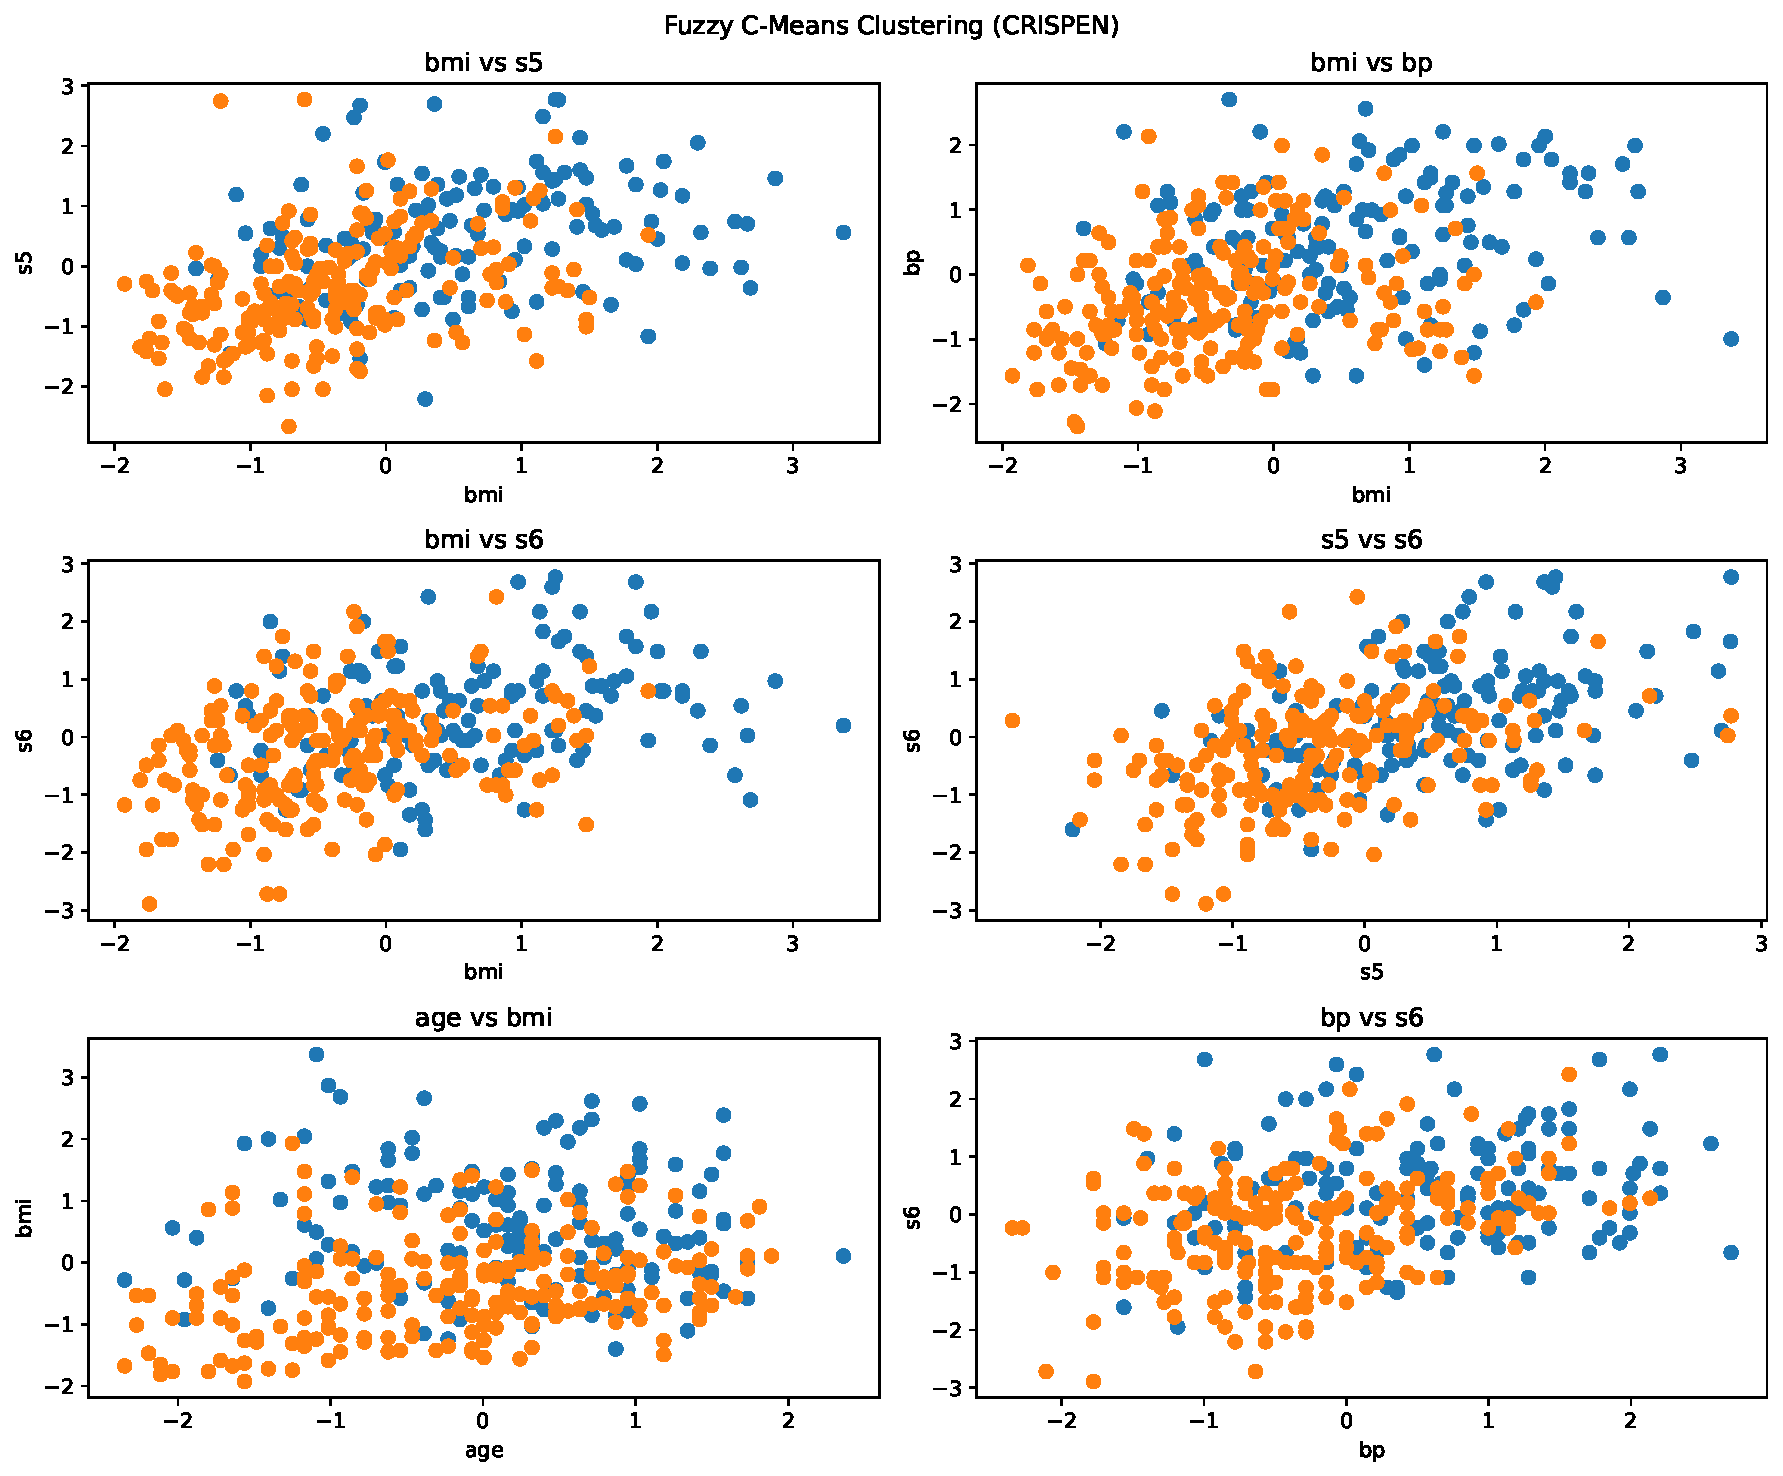
\includegraphics[width=1\textwidth]{Plots/Fuzzy C-Means Clustering (CRISPEN) REG.pdf}
    \caption{Fuzzy C-Means Clustering (CRISPEN)}
    \label{fig:my_label}
\end{figure}